\documentclass[a4paper]{oblivoir}
\usepackage{amsmath,amssymb,kotex,mdframed,paralist}
\usepackage{fapapersize}
\usefapapersize{210mm,297mm,20mm,*,20mm,*}

\usepackage{tabto,pifont}
\TabPositions{0.2\textwidth,0.4\textwidth,0.6\textwidth,0.8\textwidth}

%%% 객관식 선지
\newcommand\one{\ding{172}}
\newcommand\two{\ding{173}}
\newcommand\three{\ding{174}}
\newcommand\four{\ding{175}}
\newcommand\five{\ding{176}}
\usepackage{tabto,pifont}
%\TabPositions{0.2\textwidth,0.4\textwidth,0.6\textwidth,0.8\textwidth}

\newcommand\taba[5]{\par\noindent
\one\:{#1}
\tabto{0.2\textwidth}\two\:\:{#2}
\tabto{0.4\textwidth}\three\:\:{#3}
\tabto{0.6\textwidth}\four\:\:{#4}
\tabto{0.8\textwidth}\five\:\:{#5}}

\newcommand\tabb[5]{\par\noindent
\one\:{#1}
\tabto{0.33\textwidth}\two\:\:{#2}
\tabto{0.67\textwidth}\three\:\:{#3}\medskip\par\noindent
\four\:\:{#4}
\tabto{0.33\textwidth}\five\:\:{#5}}

\newcommand\tabc[5]{\par\noindent
\one\:{#1}
\tabto{0.5\textwidth}\two\:\:{#2}\medskip\par\noindent
\three\:\:{#3}
\tabto{0.5\textwidth}\four\:\:{#4}\medskip\par\noindent
\five\:\:{#5}}

\newcommand\tabd[5]{\par\noindent
\one\:{#1}\medskip\par\noindent
\two\:\:{#2}\medskip\par\noindent
\three\:\:{#3}\medskip\par\noindent
\four\:\:{#4}\medskip\par\noindent
\five\:\:{#5}}

\usepackage{graphicx}

%\pagestyle{empty}

%%% Counters
\newcounter{num}

%%% Commands
\newcommand{\prob}[1]
{\bigskip\bigskip\noindent\refstepcounter{num}\textbf{문제 \arabic{num})} #1\par\noindent}

\newcommand\pb[1]{\ensuremath{\fbox{\phantom{#1}}}}

\newcommand\ba{\ensuremath{\:|\:}}

\newcommand\vs[1]{\par\vspace{30pt}}

\newcommand\an[1]{\bigskip\par\noindent\textbf{문제 #1)}\par\noindent}

%%% Meta Commands
\let\oldsection\section
\renewcommand\section{\clearpage\oldsection}

\let\emph\textsf

\begin{document}
\begin{center}
\LARGE태희, 미니테스트 03
\end{center}
\begin{flushright}
날짜 : 2018년 \(\pb3\)월 \(\pb{10}\)일 \(\pb{월}\)요일
,\qquad
제한시간 : \pb{17년}분
,\qquad
점수 : \pb{20} / \pb{20}
\end{flushright}

%
\prob{\(A\), \(B\), \(C\), \(D\) 네 명의 학생이 수학 시험을 보고 서로 답안지를 바꿔서 채점하기로 하였다.
네 명 모두가 다른 사람의 답안지를 채점하는 경우의 수를 구하여라.}
\taba4689{10}
\vs

%
\prob{집합 \(X=\{1,2,3,4\}\)에 대하여 \(f(x)\neq x\)를 만족시키는 함수 \(f:X\to X\)의 개수를 구하여라.}
\taba4689{10}
\vs

%
\prob{6개의 문자 \(a\), \(b\), \(c\), \(d\), \(e\), \(f\)를 일렬로 나열할 때, 다음 경우의 수를 구하여라.}
\begin{enumerate}[(1)]
\item
\(a\)가 맨 앞에, \(b\)가 맨 뒤에 오는 경우
\item
\(a\)와 \(b\) 사이에 3개의 문자가 들어 있는 경우
\end{enumerate}
\vs

%
\prob{1에서 10까지의 자연수가 각각 적혀 있는 10장의 카드에서 두 장을 뽑을 때, 적어도 한 장은 짝수가 적혀있는 카드를 뽑는 방법의 수를 구하여라.}
\taba{20}{25}{30}{35}{40}
\vs

%%
%\prob{\(A\), \(B\)를 포함한 8명 중에서 \(A\), \(B\)를 포함하여 4명을 뽑아 일렬로 세울 때, \(A\), \(B\)가 이웃하여 서는 방법의 수를 구하시오.}
%\taba{144}{288}{432}{864}{1440}
%\vs

%
\prob{집합 \(X=\{1,2,3,4,5\}\)에서 집합 \(Y=\{1,2,3,4,5,6,7,8\}\)로의 함수 \(f\)가 \(x_1<x_2\)이면 \(f(x_1)<f(x_2)\)이고 \(f(4)=6\)을 만족시킬 때, 함수 \(f\)의 개수를 구하시오.
(단, \(x_1\in X\), \(x_2\in X\))}
\vs

\noindent
\begin{minipage}{.8\textwidth}
%
\prob{
오른쪽 그림과 같이 정삼각형의 변 위에 같은 간격으로 9개의 점이 있다.
이들 점 중에서 3개의 점을 꼭짓점으로 하는 삼각형의 개수를 구하시오.}
\taba{36}{48}{60}{72}{84}
\end{minipage}
\begin{minipage}{.2\textwidth}
\centering
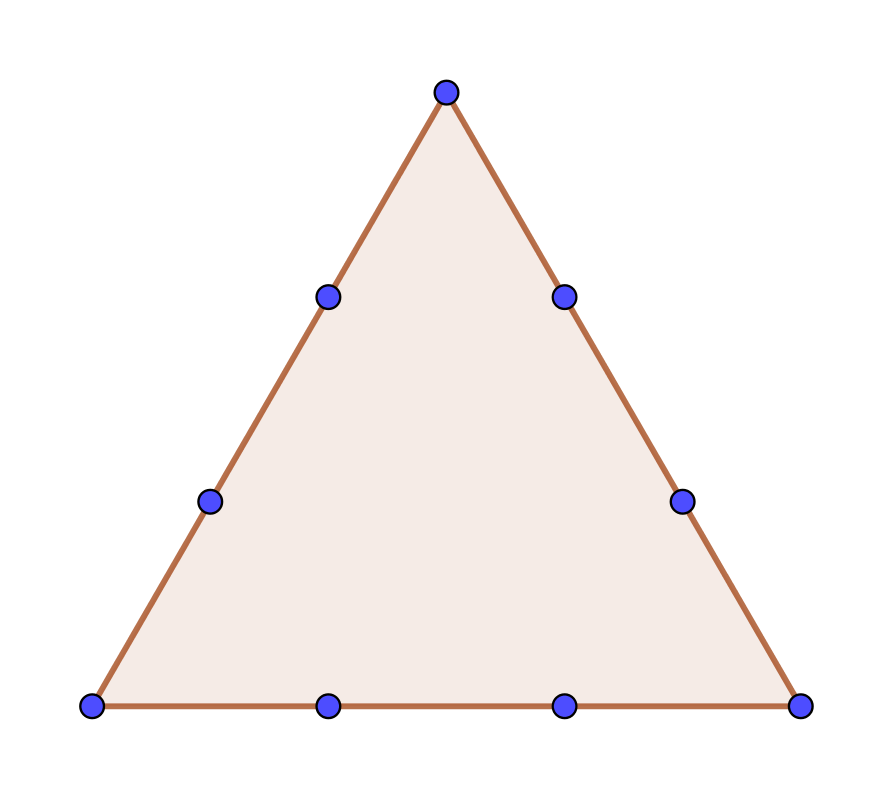
\includegraphics[width=.7\textwidth]{9points}
\end{minipage}
\vs

%%
%\prob{}
%\taba{36}{48}{60}{72}{84}

\newpage
%
\prob{7명의 학생을 2명, 2명, 3명의 세 조로 나누는 방법의 수를 구하여라.}
\taba{90}{105}{120}{135}{150}
\vspace{20pt}

%
\prob{다음 중 옳은 것은?}
\tabd
{25의 제곱근은 5이다.}
{81의 네제곱근 중 실수인 것은 3이다.}
{제곱근 9는 \(\pm3\)이다.}
{\(-1\)의 제곱근은 \(-1\)이다.}
{\(-27\)의 세제곱근 중 실수인 것은 \(-3\)이다.}
\vspace{30pt}

%
\prob{\(\displaystyle
\left(\frac{27}5\right)^{\frac12}
\times
\left\{\left(\frac{27}{125}\right)^{-\frac13}\right\}^{\frac32}
\)
의 값은?}
\taba{\(\sqrt3\)}{\(\sqrt5\)}3{\(2\sqrt3\)}5
\vs

%
\prob{\(\displaystyle
\sqrt{\sqrt[4]a}\times\sqrt{a\sqrt{a\sqrt a}}
\)
의 값은?
}
\taba{\(a^{\frac38}\)}{\(a^{\frac58}\)}{\(a^{\frac78}\)}{\(a\)}{\(a^{\frac{64}7}\)}
\vs

%
\prob{\(\displaystyle
\left\{2^{\sqrt2}+(\sqrt2)^{\sqrt2}\right\}
\left\{2^{\sqrt2}-(\sqrt2)^{\sqrt2}\right\}\)
을 간단히 하면?}
\taba{\(2^{\sqrt2}(2^{\sqrt2}-1)\)}{\(2^{\sqrt2}(2^{\sqrt2}-1)\)}{\(2^{\sqrt2}-1\)}{\((\sqrt2)^{\sqrt2}-1\)}2
\vs

%
\prob{\(a^{\frac13}+a^{-\frac13}=\sqrt5\)일 때,
\(\displaystyle\frac{a-a^{-1}}{a+a^{-1}}\)의 값은?
(단, \(a>1\))}
\taba{\(-\frac{2\sqrt5}5\)}{\(-\frac{\sqrt5}5\)}{\(\frac{\sqrt5}5\)}{\(\frac{2\sqrt5}5\)}{\(\frac{3\sqrt5}5\)}

\end{document}